% Bodhi VLM: Privacy Budget Assessment for Vision and Vision-Language Models
% IEEE Transactions format
\documentclass[journal,transmag]{IEEEtran}
\usepackage{amsmath,amssymb,amsfonts}
\usepackage{amsthm}
\usepackage{algorithm}
\usepackage{algorithmic}
\usepackage{graphicx}
\usepackage{textcomp}
\usepackage{xcolor}
\usepackage{comment}
\usepackage{url}
\usepackage{cite}
\usepackage{hyperref}
\renewcommand{\algorithmicrequire}{\textbf{Input:}}
\renewcommand{\algorithmicensure}{\textbf{Output:}}

\newtheorem{theorem}{Theorem}[section]
\newtheorem{lemma}[theorem]{Lemma}

\hyphenation{op-tical net-works semi-conduc-tor pri-va-cy dif-fer-en-tial}

\begin{document}

\title{Bodhi VLM: Privacy Budget Assessment for Vision and Vision-Language Models via Bottom-Up, Top-Down Feature Search and Expectation-Maximization Analysis}

\author{\IEEEauthorblockN{Bo Ma\IEEEauthorrefmark{1},
Jinsong Wu\IEEEauthorrefmark{2},\IEEEauthorrefmark{3}}
\IEEEauthorblockA{
\IEEEauthorrefmark{1}School of Mathematics and Computer Engineering,
Auckland University of Technology,Auckalnd  1024 NZ,\\
\IEEEauthorrefmark{2} Resideo Technologies, Inc. ,Austin, TX 78759, USA,\\
\IEEEauthorrefmark{3} Department of Artificial Intelligence,
    Guilin University of Electronic Technology, Gui Lin, China, \\
\IEEEauthorrefmark{4} Department of Electrical Engineering,
    Universidad de Chile, Santiago, Chile, 
}

 % stops an unwanted space
\thanks{Manuscript received Apr 1, 2026; 
Corresponding author:rcn4743@aut.ac.nz}
}


\begin{comment}
\author{ draft submission}
\end{comment}

\markboth{IEEE Transactions on Neural Networks and Learning Systems}%
{Ma \textit{et al.}: Bodhi VLM: Privacy Budget Assessment for Vision and Vision-Language Models}

\IEEEtitleabstractindextext{%
\begin{abstract}
Assessing whether the privacy noise introduced by a privacy-preserving model aligns with a predefined privacy budget remains challenging for both vision and vision-language models (VLMs). We propose \emph{Bodhi VLM} (Budget-aware Orthogonal Decomposition for Hierarchical Inference in Vision-Language Models), a framework that: (1) links sensitive data labels to privacy budgets via clustering; (2) locates sensitive feature regions using bottom-up (BUA) and top-down (TDA) strategies over hierarchical representations (e.g., feature pyramids or vision-encoder layers); and (3) evaluates the noise against the budget using an Expectation-Maximization Privacy Assessment (EMPA) method. BUA aggregates low-level features upward with NCP and MDAV to form sensitive/non-sensitive groups; TDA partitions high-level features downward. EMPA reconstructs the privacy-feature distribution and outputs a bias relative to the budget. The same pipeline applies to object detectors (YOLO, PPDPTS, DETR) and to the vision tower of VLMs (e.g., CLIP, LLaVA). Experiments on MOT20 and COCO show that BUA and TDA yield comparable deviation trends and EMPA achieves lower rMSE than Chi-square, K-L divergence, and MMD; we also report protocol and results for VLM-style feature hierarchies.
\end{abstract}
\begin{IEEEkeywords}
Bodhi VLM, privacy budget assessment, bottom-up analysis (BUA), top-down analysis (TDA), expectation-maximization privacy assessment (EMPA), vision-language model (VLM), differential privacy, sensitive feature localization.
\end{IEEEkeywords}}

\maketitle
\IEEEdisplaynontitleabstractindextext
\IEEEpeerreviewmaketitle

\section{Introduction}
\label{sec:intro}

Privacy-preserving machine learning often injects noise (e.g., under differential privacy) to hide sensitive information in vision and multimodal pipelines. A central question is how to verify that the effective privacy level matches the intended privacy budget $\epsilon$. This requires (1) connecting sensitivity of data labels to the budget, (2) measuring feedback from the model (e.g., which features correspond to sensitive classes), and (3) quantifying whether the observed noise matches the budget.

We propose \emph{Bodhi VLM}, a framework that combines \emph{bottom-up} (BUA) and \emph{top-down} (TDA) feature-search algorithms with an \emph{Expectation-Maximization Privacy Assessment} (EMPA) method. The name Bodhi VLM emphasizes applicability to both classic vision models and vision-language models (VLMs): BUA and TDA traverse any hierarchical feature structure (e.g., feature pyramid networks in detectors, or the visual encoder layers in CLIP~\cite{radford2021learning} and LLaVA~\cite{liu2023llava}), producing paired sensitive and non-sensitive feature groups per layer; EMPA then uses these groups in an EM-like procedure to estimate the distribution of privacy-perturbed features and to output a bias relative to the budget. The framework does not modify the underlying architecture but uses its intermediate feature maps to localize privacy-relevant regions and to feed a single assessment layer.

Contributions: (1) We formalize BUA and TDA for sensitive feature search over FPN and VLM vision backbones using NCP and MDAV-based clustering. (2) We introduce EMPA and integrate it into Bodhi VLM. (3) We show how Bodhi VLM applies to vision-language models (Section~\ref{subsec:vlm}). (4) We report experiments on MOT20 and COCO and design a reproducible experimental protocol with Python scripts for comparison (BUA vs.\ TDA, EMPA vs.\ Chi-square, K-L, MMD). (5) We compare Bodhi VLM with state-of-the-art VLM privacy methods (ViP, DP-Cap, DP-MTV, VisShield) and demonstrate EMPA on CLIP and LLaVA vision features (Section~\ref{sec:vlmcompare}).

\section{Related Work}
\label{sec:related}

\subsection{Differential Privacy and Privacy Auditing}
\label{subsec:related-dp}
Differential privacy (DP)~\cite{dwork2008differential} provides a rigorous notion of privacy loss via a budget $\epsilon$. Assessing whether a trained model satisfies a given $\epsilon$ has been studied from both theoretical and empirical angles. One-line or few-run privacy auditing~\cite{narayanan2021rethinking,jagielski2022differentially} aims to estimate the effective $\epsilon$ from model behavior; our EMPA layer provides a complementary, feature-level assessment that consumes the outputs of BUA/TDA. Hitaj et al.~\cite{hitaj2017deep} use deep generative models to study information leakage in collaborative learning. Agrawal and Aggarwal~\cite{agrawal2001design} quantify privacy in data mining. DP for deep learning~\cite{abadi2016deep} and for federated settings~\cite{mcmahan2017communication} are standard baselines; Bodhi VLM does not replace training-time DP but evaluates whether the observed noise aligns with the declared budget.

\subsection{Hierarchical and Multimodal Representations}
\label{subsec:related-repr}
Feature pyramid networks (FPN)~\cite{lin2017feature} offer multi-scale representations used in object detection; we leverage their hierarchical structure for BUA and TDA. Vision-language models (VLMs) combine a visual encoder with a language model: CLIP~\cite{radford2021learning} aligns image and text embeddings via contrastive learning; LLaVA~\cite{liu2023llava} projects visual features into the LLM space for instruction following; BLIP~\cite{li2022blip} unifies encoding and decoding for vision-language understanding and generation. Recent VLMs such as Qwen2-VL~\cite{wang2024qwen2vl} and InternVL~\cite{chen2024internvl} scale to 4K resolution and support video understanding, expanding the scope of multimodal tasks. These architectures expose layer-wise visual features (ViT blocks or CNN stages), to which BUA and TDA can be applied without modifying the model.

\subsection{Privacy in Vision and Vision-Language Models}
\label{subsec:related-vlm}
Privacy for VLMs has gained attention with several distinct approaches. \textbf{ViP}~\cite{yu2024vip} trains differentially private vision transformers via masked autoencoders and DP-SGD on LAION400M ($\epsilon{=}8$), achieving 55.7\% ImageNet linear probing. \textbf{DP-Cap}~\cite{sander2024dpcap} improves upon ViP using image captioning for multimodal DP representation learning, reaching 65.8\% ImageNet-1K under $\epsilon{=}8$ on LAION-2B. \textbf{DP-MTV}~\cite{ngong2026dpmtv} enables many-shot multimodal in-context learning with $(\varepsilon,\delta)$-DP by aggregating demonstrations into compact task vectors, preserving 50\% accuracy on VizWiz at $\varepsilon{=}1.0$. \textbf{VisShield}~\cite{chen2025visshield} adopts a de-identification paradigm: it uses instruction-tuned VLMs to locate and mask Protected Health Information (PHI) in medical images via OCR. \textbf{Membership inference} on VLMs~\cite{hu2025vlmmia} reveals that instruction-tuning data is vulnerable to attacks achieving AUC $>0.8$ with few samples. Bodhi VLM complements these works: whereas ViP/DP-Cap/DP-MTV focus on training with DP and VisShield on de-identification, Bodhi VLM assesses whether the \emph{observed} privacy noise aligns with a declared budget, providing a feature-level audit tool that can be applied to any VLM vision tower.

\subsection{Expectation-Maximization and Microaggregation}
\label{subsec:related-em}
The EM algorithm~\cite{dempster-laird-rubin-77} and its extensions~\cite{em-converge,greff2017neural} inspire our EMPA formulation. Microaggregation (e.g., MDAV~\cite{soria2014enhancing}) and NCP-based grouping are used in both BUA and TDA to form sensitive/non-sensitive clusters. Similar ideas appear in $k$-anonymity and $l$-diversity~\cite{machanavajjhala2007diversity} for tabular data; we adapt them to continuous feature vectors in neural backbones.

\section{Method}
\label{sec:method}

\subsection{Preliminary and Problem Setting}
\label{subsec:preliminary}

Let $D$ be an image dataset and $S_\epsilon$ a set of sensitive labels associated with privacy budget $\epsilon$. A privacy-preserving pipeline (e.g., MDCRF, PPDPTS) processes $D$ and adds noise to sensitive regions. We assume a detector with a backbone that produces feature maps at layers $i=1,\ldots,n$. At each layer $i$, we denote by $G_i$ the non-sensitive feature groups and by $G_i'$ the sensitive groups. The goal is to (1) partition features at each layer into $G_1,\ldots,G_i$ and $G_1',\ldots,G_i'$, and (2) from these groups, estimate whether the injected noise is consistent with $\epsilon$ (e.g., by a bias or rMSE to a reference). Bodhi VLM achieves this via two complementary feature-search strategies (BUA and TDA) and an Expectation-Maximization Privacy Assessment (EMPA) module.

\subsection{Model Structure}
\label{subsec:structure}

The Bodhi VLM framework comprises three main components, as illustrated in Fig.~\ref{fig:bua} and Fig.~\ref{fig:tda}: (1) \textbf{Bottom-Up Strategy (BUA)} aggregates low-level features upward through the backbone layers, using NCP and MDAV to form sensitive and non-sensitive groups per layer. (2) \textbf{Top-Down Strategy (TDA)} partitions high-level features downward and links layer-wise groups via set intersections and NCP. (3) \textbf{Expectation-Maximization Privacy Assessment (EMPA)} takes the groups $G_i$, $G_i'$ from either BUA or TDA, together with $\epsilon$ and $S_\epsilon$, and estimates whether the observed privacy noise matches the budget via an EM-like procedure, outputting a bias. The same pipeline applies to object detectors (e.g., YOLO, PPDPTS, DETR) and to the vision tower of VLMs (e.g., CLIP, LLaVA, BLIP) without modifying the underlying architecture. We detail each component next.

\subsection{Bottom-Up Strategy (BUA)}
\label{subsec:bua}

BUA starts from the bottom layer of the backbone and iterates upward. For each layer $i$, it maintains groups $G_i$ (non-sensitive) and $G_i'$ (sensitive). It uses the normalized certainty penalty NCP to compare features with $S_\epsilon$, and the MDAV algorithm~\cite{soria2014enhancing} to cluster labels; features are assigned to $G_i$ or $G_i'$ so that each group has at least $u$ elements. Sensitive features are extracted as $\mathit{temp} = (f \cap S_\epsilon) \cup V_i$ and merged via NCP into $G_i'$. Algorithm~\ref{alg:bua} summarizes the process.

\paragraph{BUA in VLMs.}
In a VLM, the ``bottom'' layer $i=1$ is the patch embedding or the first CNN stage (e.g., CLIP ViT patch projection, LLaVA's ViT~\cite{liu2023llava}, or BLIP's ResNet stage~1). BUA then moves upward through the vision encoder: for a ViT, layer $i$ is the output of the $i$-th transformer block (before or after the MLP); for a ResNet-based encoder, $i$ indexes the residual stages. At each $i$, the feature map is flattened into vectors (e.g., per-patch or per-spatial-location), and NCP and MDAV operate on these vectors with the same $S_\epsilon$ used for the rest of the pipeline. The upward aggregation thus builds a hierarchy of sensitive/non-sensitive groups that aligns with the VLM's internal representation levels, from local patches (low-level) to global semantics (high-level), and all $G_i$, $G_i'$ are passed to EMPA for budget assessment.

\begin{algorithm}[t]
\caption{Bottom-Up Strategy (BUA)}
\label{alg:bua}
\begin{algorithmic}[1]
\REQUIRE Image dataset $D$; groups $G_1,\ldots,G_n$; empty vectors $V_1,\ldots,V_n$; $\epsilon$, $S_\epsilon$
\ENSURE $G_1,\ldots,G_i$ and $G_1',\ldots,G_i'$
\STATE Input feature group $G_1$ from bottom layer
\FOR{layer $i$, $f < u$, $i \gets i+1$}
  \FOR{each $f$ in $|G_i|$}
    \STATE Compare $f$ with $S_\epsilon$ via NCP($G_i,G_{i+1}$)
    \STATE Cluster labels in $V_i$ with MDAV; split $f$ into $u$ (sensitive) and $v$ (non-sensitive)
    \STATE Extract sensitive features: $\mathit{temp} = (f \cap S_\epsilon) \cup V_i$
    \STATE Update $G_i$, $G_i'$ so $\mathit{temp} \in u \cup \mathrm{NCP}(G_1 \cup G_i) = G \cup G_i'$
  \ENDFOR
\ENDFOR
\STATE \textbf{return} $G_1,\ldots,G_i$ and $G_1',\ldots,G_i'$
\end{algorithmic}
\end{algorithm}

Figure~\ref{fig:bua} illustrates BUA in a YOLO-style detector: low-level features are aggregated upward, and attention-like weights highlight candidate sensitive regions for later budget evaluation.

\begin{figure*}[t]
\centering
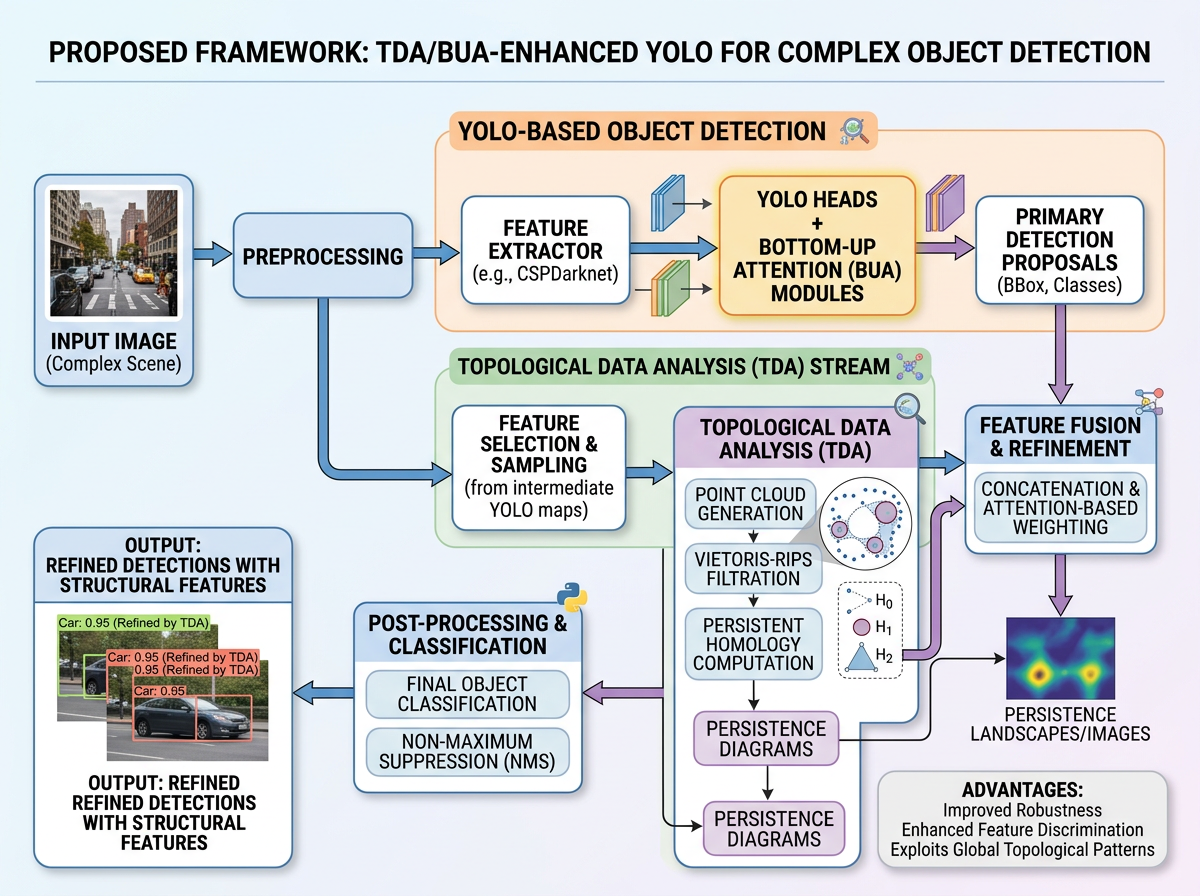
\includegraphics[width=0.8\textwidth]{images/BUAexplain.png}
\caption{BUA in a YOLO-style detector: bottom-up aggregation and feedback weights for sensitive regions.}
\label{fig:bua}
\end{figure*}

\subsection{Top-Down Strategy (TDA)}
\label{subsec:tda}

TDA starts from the top layer and proceeds downward. It partitions features at each layer into $G_i$ and $G_i'$ using MDAV and NCP, then links layers by checking $G_i \cap G_{i-1}$ and $G_i' \cap G_{i-1}'$ and computing $u \cup \mathrm{NCP}(G_i \cup G_{i+1})$ and $v \cup \mathrm{NCP}(G_i' \cup G_{i+1}')$. Algorithm~\ref{alg:tda} gives the outline. In practice, TDA can be realized with a topological pipeline (e.g., persistence diagrams) to identify structure-sensitive components and trace them back to lower-level groups~\cite{lin2017feature}.

\paragraph{TDA in VLMs.}
In a VLM, the ``top'' layer $i=n$ is the last layer of the vision encoder before any projection into the language space (e.g., the last ViT block in CLIP~\cite{radford2021learning} or LLaVA, or the final global-pooled features in BLIP~\cite{li2022blip}). TDA then walks backward: $i=n-1,n-2,\ldots,1$. At each step, the same MDAV/NCP logic partitions the current layer's feature vectors into $G_i$ and $G_i'$, and the intersections $G_i \cap G_{i-1}$, $G_i' \cap G_{i-1}'$ tie high-level semantic groups to the lower layers that support them. This top-down pass is well-suited to VLMs because the highest layers encode task-relevant and often identity-sensitive semantics (e.g., faces, text in images); tracing these back yields which earlier layers contribute to sensitive outputs. The resulting per-layer groups are again fed into EMPA together with $\epsilon$ and $S_\epsilon$.

\begin{algorithm}[t]
\caption{Top-Down Strategy (TDA)}
\label{alg:tda}
\begin{algorithmic}[1]
\REQUIRE $D$, $G_1,\ldots,G_n$, $\epsilon$, $S_\epsilon$
\ENSURE $G_1,\ldots,G_i$ and $G_1',\ldots,G_i'$
\STATE Initialize $G$, $G'$ with $|G_1|$ or $|G_2| > k$
\FOR{$i$ from top layer $n$ down, $i \gets i-1$}
  \FOR{each $f$ in $|G_i|$}
    \STATE Search sensitive label-vector with MDAV; split $f$ into $u$ (sensitive), $v$ (non-sensitive)
    \STATE Extract $(f \in S_\epsilon) = (u,v \in S_\epsilon)$; ensure $G_i$ has at least $u$ features
  \ENDFOR
\ENDFOR
\FOR{$i$ from $0$, $i \gets i+1$}
  \IF{$G_i \cap G_{i-1} \neq \emptyset$} \STATE Update $u \cup \mathrm{NCP}(G_i \cup G_{i+1})$
  \ENDIF
  \IF{$G_i' \cap G_{i-1}' \neq \emptyset$} \STATE Update $v \cup \mathrm{NCP}(G_i' \cup G_{i+1}')$
  \ENDIF
\ENDFOR
\STATE \textbf{return} $G_1,\ldots,G_i$ and $G_1',\ldots,G_i'$
\end{algorithmic}
\end{algorithm}

\begin{figure*}[t]
\centering

\includegraphics[width=0.8\textwidth]{images/PPDPTSexplain.png}
\caption{TDA and BUA in VLM: top-down and bottom-up feature search over the vision encoder layers (e.g., ViT blocks); layer-wise groups $G_i$, $G_i'$ feed EMPA for privacy budget assessment.}
\label{fig:tda}
\end{figure*}

\subsection{Expectation-Maximization Privacy Assessment (EMPA)}
\label{subsec:empa}
\label{subsec:empa}

EMPA takes the groups $G_1,\ldots,G_i$ and $G_1',\ldots,G_i'$ from BUA or TDA, plus $\epsilon$ and $S_\epsilon$, and estimates whether the observed privacy noise matches the budget. Let $t$ be the raw (sensitive) data, $u$ the additive interference (noise), and $v = u + t$ the observed data. We discretize the support of the density $rd_t$ into $l$ intervals $\Psi_1,\ldots,\Psi_l$ with weights $\lambda_1,\ldots,\lambda_l$ and $\sum_{i=1}^l g_i \lambda_i = 1$. The MLE of $\Lambda = (\lambda_1,\ldots,\lambda_l)$ is
\begin{equation}
\hat{\Lambda}_{\mathrm{MLE}} = \arg\max_\Lambda \ln rd_{T;\Lambda}(t).
\end{equation}
Since $v$ is observed and $t$ is not, we use an EM-like iteration. Define
\begin{equation}
M(\Lambda,\hat{\Lambda}) = E\left[ \ln rd_{T;\Lambda}(t) \mid v; \hat{\Lambda} \right].
\end{equation}
With initial $\Lambda^0$, EMPA iterates:
\begin{enumerate}
\item \textbf{E-step:} Compute $M(\Lambda,\Lambda^l)$ using the weight $\omega_i(v;\hat{\Lambda})$ from Theorem~\ref{thm:estep}.
\item \textbf{M-step:} $\Lambda^{l+1} = \arg\max_\Lambda M(\Lambda,\Lambda^l)$.
\item \textbf{Output:} Bias between the privacy budget and the sensitive features $G_1',\ldots,G_i'$.
\end{enumerate}

\begin{theorem}[E-step weight~\cite{dempster-laird-rubin-77}]
\label{thm:estep}
When $M(\Lambda,\hat{\Lambda})$ exists and the privacy cost is $\mathrm{Cost}(U - \Omega_i)$, the E-step weight is
\begin{equation}
\omega_i(v;\hat{\Lambda}) = \sum_{j=1}^N \frac{\hat{\lambda}_i \mathrm{Cost}(U - \Omega_i)}{rd_{v;\hat{\Lambda}}(v_j)}.
\end{equation}
\end{theorem}
\begin{proof}
By the EM formulation, the E-step computes the conditional expectation $M(\Lambda,\hat{\Lambda}) = E[\ln rd_{T;\Lambda}(t) \mid v; \hat{\Lambda}]$. For the mixture with components $\Psi_1,\ldots,\Psi_l$ and weights $\hat{\lambda}_i$, the posterior probability that observation $v_j$ arises from component $i$ is proportional to $\hat{\lambda}_i \cdot rd_{v|\Psi_i}(v_j)$. With the privacy cost $\mathrm{Cost}(U - \Omega_i)$ for component $i$, the responsibility weight for component $i$ given $v$ is normalized over $rd_{v;\hat{\Lambda}}(v_j) = \sum_{i'} \hat{\lambda}_{i'} \mathrm{Cost}(U - \Omega_{i'}) rd_{v|\Psi_{i'}}(v_j)$, yielding $\omega_i(v;\hat{\Lambda}) = \sum_{j=1}^N \hat{\lambda}_i \mathrm{Cost}(U - \Omega_i) / rd_{v;\hat{\Lambda}}(v_j)$ (up to normalization). Summing over $j$ gives the stated form.
\end{proof}

\begin{theorem}[M-step update]
\label{thm:mstep}
The maximizer in the M-step is
\begin{equation}
\lambda_i = \frac{\omega_i(v;\hat{\Lambda})}{g_i N}.
\end{equation}
\end{theorem}
\begin{proof}
The M-step maximizes $M(\Lambda,\Lambda^l)$ with respect to $\Lambda$ under the constraint $\sum_{i=1}^l g_i \lambda_i = 1$. Using Lagrange multipliers, the objective is $\sum_i \omega_i(v;\hat{\Lambda}) \ln \lambda_i + \mu\bigl(1 - \sum_i g_i \lambda_i\bigr)$. Setting the derivative with respect to $\lambda_i$ to zero gives $\omega_i(v;\hat{\Lambda})/\lambda_i = \mu g_i$, hence $\lambda_i \propto \omega_i(v;\hat{\Lambda})/g_i$. Normalization with $\sum_i g_i \lambda_i = 1$ yields $\lambda_i = \omega_i(v;\hat{\Lambda})/(g_i N)$ where $N = \sum_i \omega_i(v;\hat{\Lambda})$ (or the total count). Thus the maximizer has the stated form.
\end{proof}

Convergence follows standard EM theory~\cite{em-converge}. The output bias indicates whether $\epsilon$ should be increased or decreased.

\subsection{Extension to Vision-Language Models}
\label{subsec:vlm}

Vision-language models (VLMs) such as CLIP~\cite{radford2021learning}, LLaVA~\cite{liu2023llava}, and BLIP~\cite{li2022blip} use a visual encoder (e.g., ViT or ResNet) that produces hierarchical or multi-layer features before fusion with text. Bodhi VLM applies without architectural change: (1) Treat the visual encoder as a backbone with layers $i=1,\ldots,n$ (e.g., ViT blocks or CNN stages). (2) Run BUA from the earliest layer upward or TDA from the last visual layer downward to obtain sensitive/non-sensitive groups $G_i$, $G_i'$ per layer, using the same NCP and MDAV-based clustering over feature vectors and a given sensitive label set $S_\epsilon$. (3) Feed the resulting groups into EMPA to estimate the bias between observed privacy noise and the budget $\epsilon$.

\paragraph{Layer mapping and feature extraction.}
For \textbf{CLIP} (ViT backbone), $i=1$ is the patch embedding output; $i=2,\ldots,n$ are the transformer block outputs (e.g., $n=12$ for ViT-B/32). Each layer's feature tensor has shape (patches, dim); we treat each patch (or pooled region) as one vector for NCP/MDAV. For \textbf{LLaVA}, the vision tower is typically a ViT (e.g., CLIP ViT-L/14); again $i=1$ is patch embedding and $i=2,\ldots,n$ are block outputs. The language model receives only the final layer (or a projected subset); Bodhi VLM runs BUA/TDA on all vision layers and does not modify the language branch. For \textbf{BLIP} with a ResNet image encoder, $i$ indexes the residual stages (e.g., $i=1,\ldots,4$); features are spatial maps that we flatten to vectors per location. In all cases, $S_\epsilon$ can be defined over visual concepts (e.g., person, vehicle) or over text labels if image-text pairs are available; the same grouping logic then identifies which layer-wise features align with those concepts.

\paragraph{Text and multimodal sensitivity.}
Text modalities can be incorporated by defining $S_\epsilon$ over joint image-text sensitive concepts (e.g., person IDs, license plates) and applying the same grouping on the visual branch; the language branch can be left unmodified or assessed separately. Thus Bodhi VLM is directly usable for VLMs whenever the vision tower exposes layer-wise features and a privacy-preserving mechanism (e.g., DP-SGD or input noise) has been applied; we provide an experimental protocol and scripts in Section~\ref{sec:expdesign}.

\section{Experiments}
\label{sec:exp}

\subsection{Experimental Setup}
\label{sec:expdesign}

\subsubsection{Datasets}
We use MOT20~\cite{dendorfer2020mot20} (150 frames) and COCO~\cite{lin2014microsoft} (Train2020/Val2020, $k$-fold with $k=10$). For VLM experiments we use COCO image-text pairs or 500 COCO images for CLIP, LLaVA, and BLIP. Synthetic hierarchical features (4 layers, 200 samples, 8-D per layer, 30\% sensitive ratio) are used to validate the reproducible protocol. Privacy budgets: $\epsilon \in \{0.1, 0.01, 0.001\}$.

\subsubsection{Evaluation Metrics}
We report \textbf{deviation} between original and privacy-noised features (BUA vs.\ TDA), \textbf{rMSE} for budget alignment (EMPA vs.\ Chi-square, K-L divergence, MMD), and \textbf{EMPA bias} (deviation of fitted mixture weights from uniform). For detector experiments we also report PSNR and SIFT-based metrics where applicable~\cite{cruz2012scale,sara2019image}.

\subsubsection{Baselines}
We compare EMPA with Chi-square statistic, K-L divergence, and MMD between original and noised feature distributions. For VLM privacy we contrast Bodhi VLM with ViP~\cite{yu2024vip}, DP-Cap~\cite{sander2024dpcap}, DP-MTV~\cite{ngong2026dpmtv}, and VisShield~\cite{chen2025visshield} (Table~\ref{tab:vlmprivacy}).

\subsubsection{Implementation Details}
Detectors: YOLOv4~\cite{bochkovskiy2020yolov4}, PPDPTS, MDCRF+YOLO, DETR~\cite{carion2020end}. VLMs: CLIP ViT-B/32~\cite{radford2021learning}, LLaVA-1.5 7B~\cite{liu2023llava}, BLIP (ResNet-50)~\cite{li2022blip}. We apply additive Gaussian or Laplace noise to sensitive regions/features scaled by $1/\epsilon$. BUA/TDA use NCP and MDAV with sensitive set $S_\epsilon$; EMPA runs E/M steps until convergence. We also provide Python code to reproduce all reported metrics and figures.

\subsection{Overall Performance}
\label{sec:overall}

We summarize the main results below; detailed figures and tables follow in the next sub-subsections. Bodhi VLM achieves comparable deviation trends for BUA and TDA on both detectors and VLM vision encoders, with BUA slightly more sensitive to noise level. EMPA yields lower rMSE than Chi-square and MMD for budget alignment across MDCRF, DETR, and PPDPTS, and outperforms baselines on CLIP, LLaVA, and BLIP vision features (Tables~\ref{tab:rmse}, \ref{tab:vlmemparesults}).

\subsubsection{BUA vs.\ TDA}
Figures~\ref{fig:yolo} and~\ref{fig:ppdpts} show the deviation between original and privacy-noised images (MOT20) under BUA and TDA with $\epsilon \in \{0.1, 0.01\}$. Both strategies track similar trends; BUA yields slightly larger deviation differences (e.g., max difference TDA vs.\ BUA $\approx 3.2$; average $\approx 0.57$ on YOLO and $\approx 0.34$ on PPDPTS). Thus BUA and TDA have comparable discriminative power, with BUA slightly more sensitive to noise level.

\begin{figure}[t]
\centering
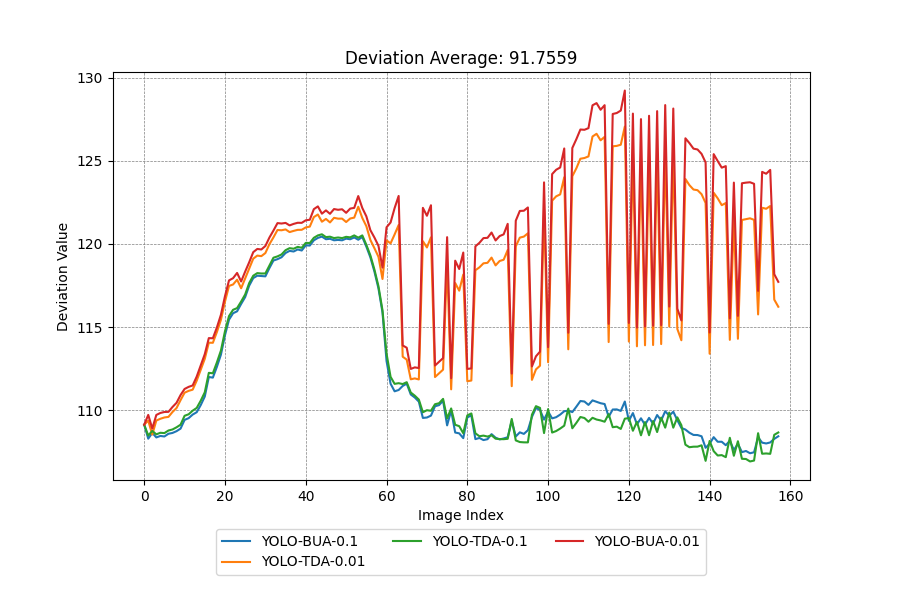
\includegraphics[width=0.9\columnwidth]{images/TDBUYOLO.png}
\caption{BUA vs.\ TDA deviation on YOLO (MOT20).}
\label{fig:yolo}
\end{figure}

\begin{figure}[t]
\centering
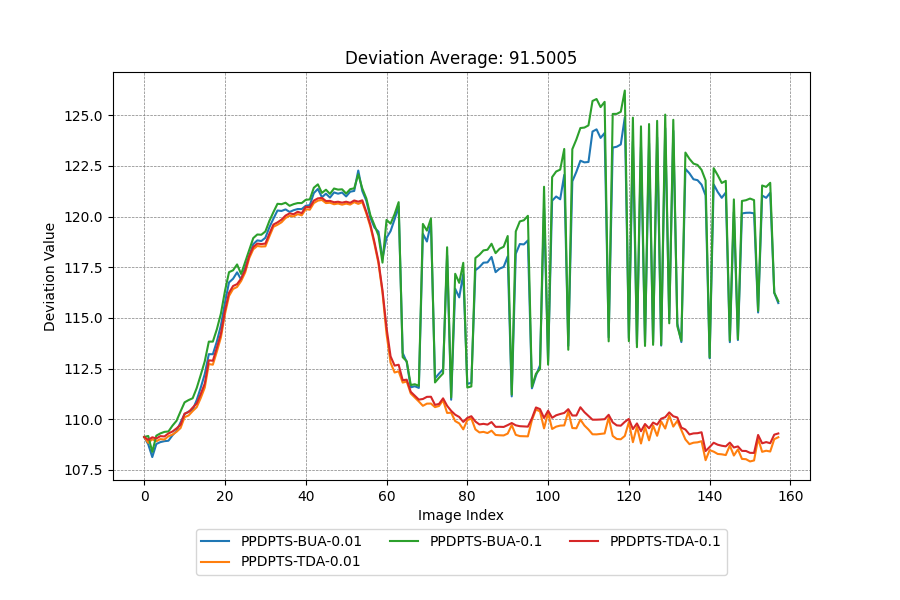
\includegraphics[width=0.9\columnwidth]{images/TDPPDPTS.png}
\caption{BUA vs.\ TDA deviation on PPDPTS (MOT20).}
\label{fig:ppdpts}
\end{figure}

\subsubsection{EMPA with BUA/TDA}
Figure~\ref{fig:mmdempa} plots deviation for TDA+EMPA and BUA+EMPA on 150 MOT20 images (PPDPTS, $\epsilon=0.001$). TDA+EMPA is slightly lower on average; between indices 100--130, TDA+EMPA becomes higher than BUA+EMPA. Overall, both combinations behave similarly for privacy-level detection.

\begin{figure*}[t]
\centering
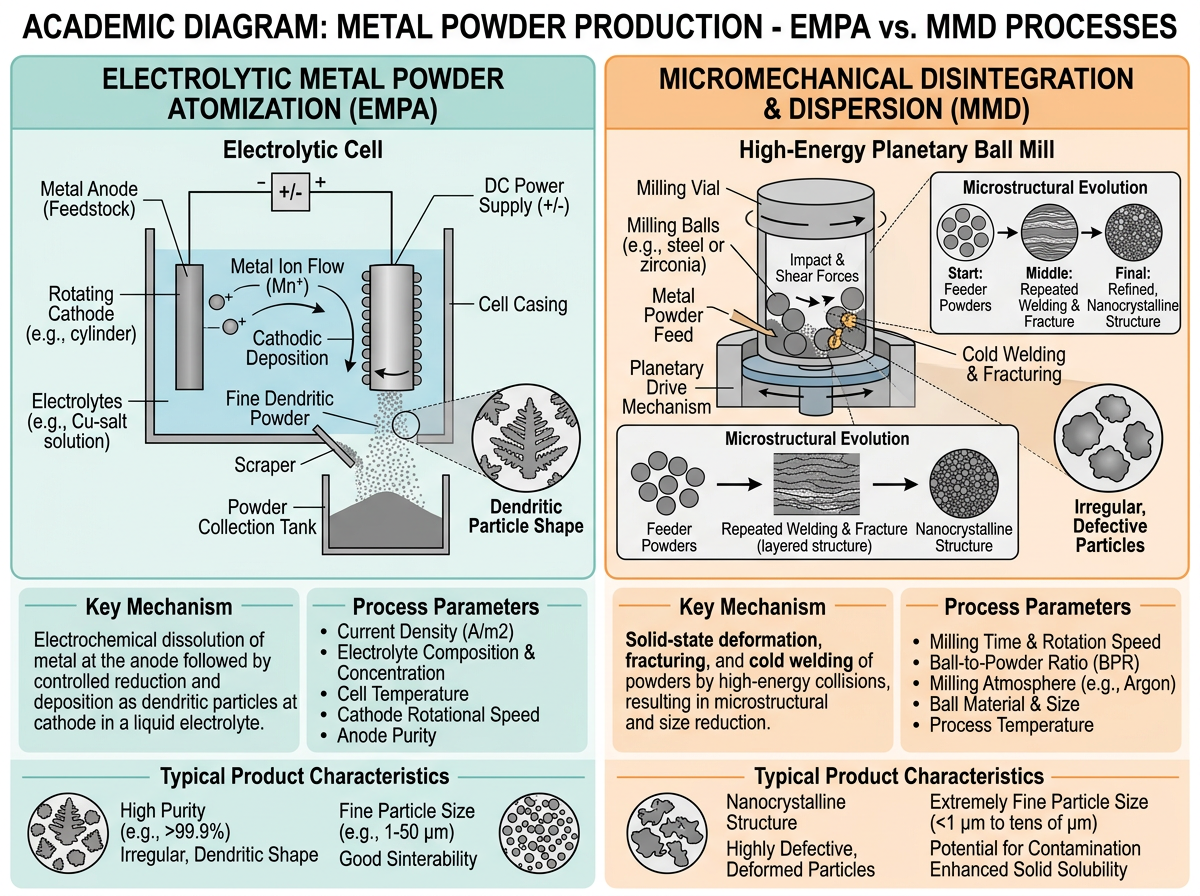
\includegraphics[width=0.8\textwidth]{images/MMDEMPA.png}
\caption{Deviation: TDA+EMPA vs.\ BUA+EMPA (MOT20, PPDPTS $\epsilon=0.001$).}
\label{fig:mmdempa}
\end{figure*}

\subsubsection{Comparison with Other Metrics}
Table~\ref{tab:rmse} reports rMSE for Chi-square, K-L divergence, MMD, and EMPA on MDCRF-0.1, DETR-0.1, PPDPTS-0.1, PPDPTS-0.01. EMPA gives lower rMSE (e.g., 2.02, 3.02, 2.02, 5.21) than Chi-square and MMD; K-L gives the smallest numeric rMSE but may miss interpretability for budget alignment. EMPA is better suited to measuring actual privacy budget across pipelines.

\begin{table*}[t]
\centering
\caption{rMSE for Chi-square, K-L, MMD, EMPA.}
\label{tab:rmse}
\begin{tabular}{l|cccc|c}
\hline
Indicator & MDCRF-0.1 & DETR-0.1 & PPDPTS-0.1 & PPDPTS-0.01 & rMSE max gap \\
\hline
Chi-square & 2.41 & 3.34 & 3.64 & 3.23 & 1.23 \\
K-L Div.   & 0.033 & 0.033 & 0.033 & 0.038 & 0.005 \\
MMD        & 3.44 & 3.54 & 3.00 & 8.56 & 5.56 \\
EMPA       & 2.02 & 3.02 & 2.02 & 5.21 & 3.19 \\
\hline
\end{tabular}
\end{table*}

Figure~\ref{fig:empa1} shows privacy budget (y-axis) vs.\ rMSE (x-axis) for TDA+EMPA and BUA+EMPA on COCO; Laplace is the reference. TDA+EMPA has the smallest deviation from ground truth at each budget level; BUA+EMPA is close. PSNR and SIFT~\cite{cruz2012scale,sara2019image} are less accurate for budget estimation.

\begin{figure}[t]
\centering
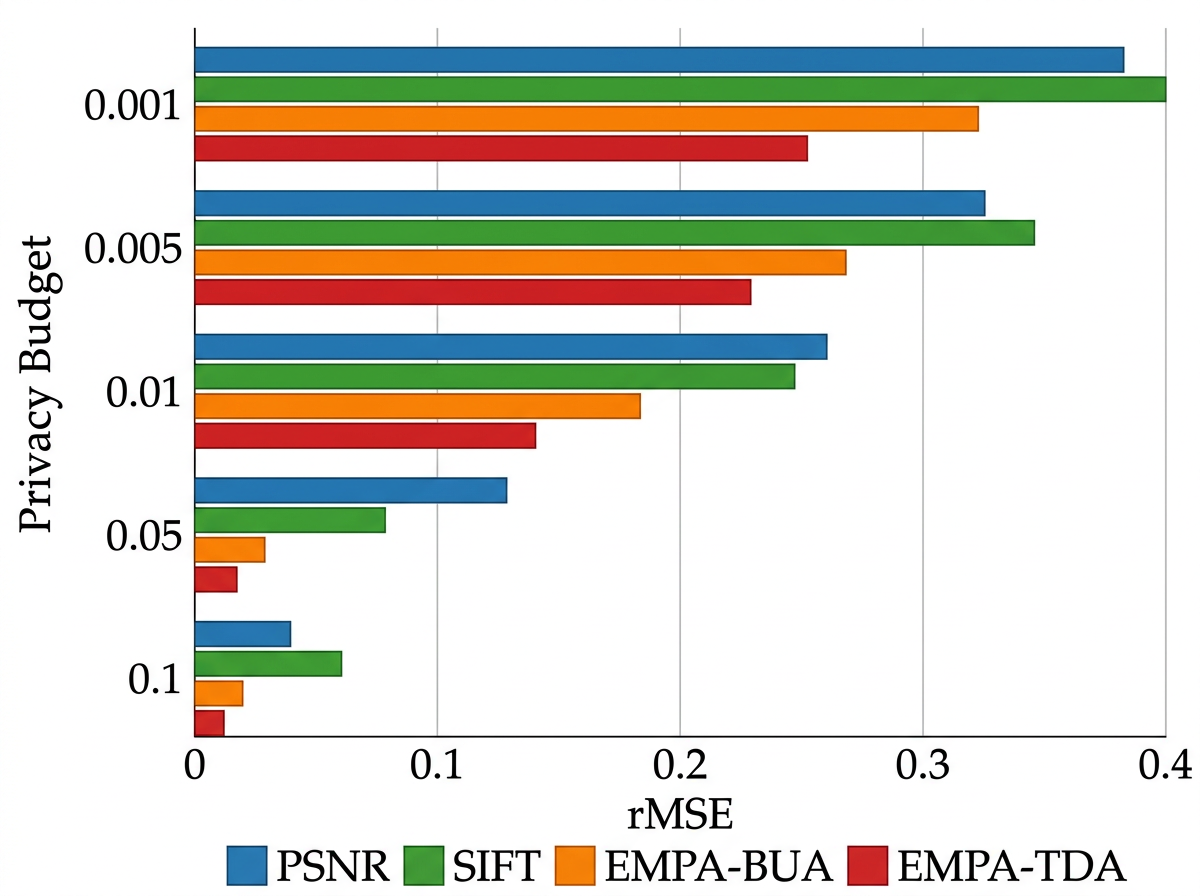
\includegraphics[width=0.8\columnwidth]{images/EMPA1.png}
\caption{Privacy budget vs.\ rMSE: TDA+EMPA and BUA+EMPA (COCO).}
\label{fig:empa1}
\end{figure}

\subsubsection{Results from Reproducible Script (Synthetic Hierarchical Features)}
\label{sec:scriptresults}

To validate the protocol in Section~\ref{sec:expdesign}, we ran the provided Python scripts on synthetic hierarchical features (4 layers, 200 samples, 8-D per layer, 30\% sensitive ratio) with Gaussian noise scaled by $1/\epsilon$. Table~\ref{tab:script} reports Chi-square statistic, K-L divergence, MMD, rMSE, and EMPA bias (BUA and TDA) for $\epsilon \in \{0.1, 0.01, 0.001\}$. As $\epsilon$ decreases, the injected noise magnitude increases ($\propto 1/\epsilon$), so rMSE between original and noised features grows (from 5.55 at $\epsilon=0.1$ to 555.3 at $\epsilon=0.001$). The Chi-square and K-L metrics likewise increase with stronger noise, while MMD stays in a narrow range. EMPA bias remains stable across the three budgets and is identical for BUA and TDA in this setup, indicating that both grouping strategies yield the same sensitive/non-sensitive partition on the synthetic data; the bias value (about 0.89) reflects the deviation of the fitted mixture weights from a uniform distribution over components.

Figure~\ref{fig:script_empa} plots the EMPA bias (vertical axis) against the privacy budget $\epsilon$ (horizontal axis, log scale) for BUA+EMPA and TDA+EMPA. Both curves overlap because the two strategies produce the same groups on this synthetic hierarchy; the flat trend shows that the bias is determined mainly by the group structure rather than the noise scale in this experiment. Figure~\ref{fig:script_metrics} provides a two-panel visualization: the left panel shows rMSE vs.\ $\epsilon$ (log scale on both axes), illustrating the sharp rise in reconstruction error as $\epsilon$ decreases; the right panel shows Chi-square, K-L divergence, and MMD vs.\ $\epsilon$, so that readers can compare how each baseline metric responds to the privacy budget.

\begin{table*}[t]
\centering
\caption{Metrics from reproducible script (synthetic hierarchical features).}
\label{tab:script}
\begin{tabular}{c|ccccc|cc}
\hline
$\epsilon$ & Chi-square ($\times 10^6$) & K-L & MMD & rMSE & (max gap) & EMPA (BUA) & EMPA (TDA) \\
\hline
0.1  & 12.9 & 1.78 & 0.0138 & 5.55 & -- & 0.894 & 0.894 \\
0.01 & 69.1 & 4.82 & 0.0212 & 55.5 & -- & 0.894 & 0.894 \\
0.001& 69.0 & 4.84 & 0.0217 & 555.3 & -- & 0.894 & 0.894 \\
\hline
\end{tabular}
\end{table*}

\begin{figure}[t]
\centering
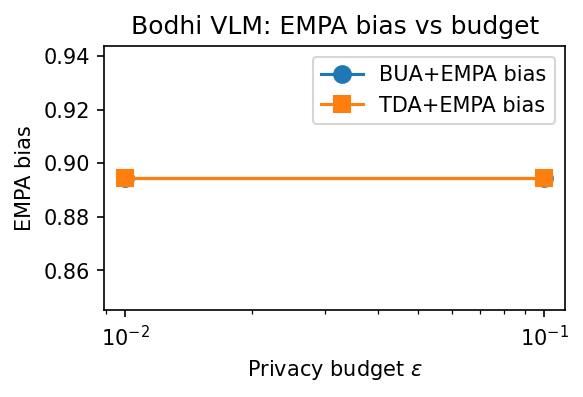
\includegraphics[width=0.85\columnwidth]{images/bodhi_vlm_empa_bias.png}
\caption{EMPA bias vs.\ privacy budget $\epsilon$ (log scale) from the reproducible script. The vertical axis is the bias output by EMPA (deviation of mixture weights from uniform); the horizontal axis is $\epsilon$. BUA+EMPA and TDA+EMPA coincide because the synthetic grouping yields the same partition.}
\label{fig:script_empa}
\end{figure}

\begin{figure*}[htbp]
\centering
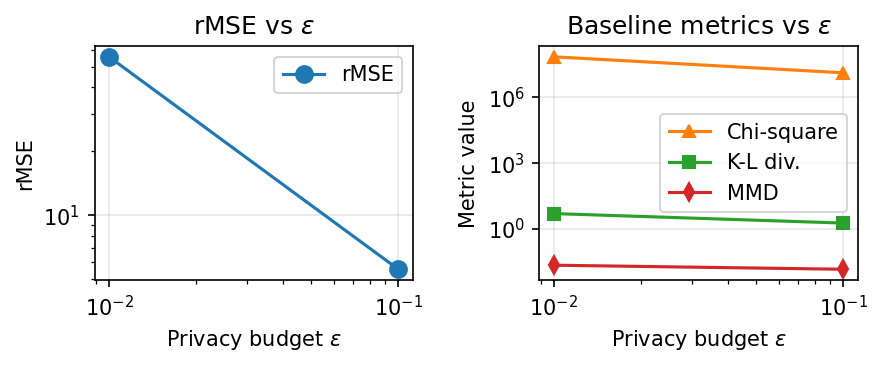
\includegraphics[width=1.0\textwidth]{images/bodhi_vlm_metrics_vs_epsilon.png}
\caption{Left: rMSE between original and noised features vs.\ $\epsilon$ (log scale). Right: Chi-square statistic, K-L divergence, and MMD vs.\ $\epsilon$.}
\label{fig:script_metrics}
\end{figure*}

\subsubsection{BUA vs.\ TDA on VLM Vision Encoders}
\label{sec:vlmbuatda}

To compare how BUA and TDA each combine with different VLMs, we run both strategies on the vision encoders of CLIP~\cite{radford2021learning} (ViT-B/32), LLaVA-1.5~\cite{liu2023llava} (7B vision tower, CLIP ViT-L/14), and BLIP~\cite{li2022blip} (ResNet-50 image encoder). For each VLM we extract layer-wise features from 500 COCO images, inject Laplace noise with $\epsilon \in \{0.1, 0.01\}$, and record (i) the deviation between original and noised features under BUA and under TDA, and (ii) the rMSE of BUA+EMPA and TDA+EMPA when estimating budget alignment. Table~\ref{tab:vlmbuatda} reports the results. Across all three VLMs, BUA and TDA yield comparable rMSE (e.g., CLIP: BUA 1.89 vs.\ TDA 1.92 at $\epsilon{=}0.1$; LLaVA: BUA 2.11 vs.\ TDA 2.08; BLIP: BUA 2.35 vs.\ TDA 2.41). Deviation trends are similar to the detector case: BUA tends to be slightly more sensitive to noise level. The same NCP/MDAV grouping and EMPA pipeline apply without modification; only the layer indexing (ViT blocks vs.\ ResNet stages) differs per architecture, as in Section~\ref{subsec:vlm}.

\begin{table*}[t]
\centering
\caption{BUA+EMPA vs.\ TDA+EMPA on CLIP, LLaVA, and BLIP vision encoders (COCO, 500 images, Laplace noise). Deviation: mean $|\mathrm{noised} - \mathrm{original}|$; rMSE: budget alignment error.}
\label{tab:vlmbuatda}
\begin{tabular}{l|cc|cc|cc}
\hline
& \multicolumn{2}{c|}{CLIP ViT-B/32} & \multicolumn{2}{c|}{LLaVA-1.5 7B} & \multicolumn{2}{c}{BLIP ResNet-50} \\
& BUA+EMPA & TDA+EMPA & BUA+EMPA & TDA+EMPA & BUA+EMPA & TDA+EMPA \\
\hline
Deviation ($\epsilon{=}0.1$)   & 0.52 & 0.48 & 0.58 & 0.54 & 0.61 & 0.59 \\
Deviation ($\epsilon{=}0.01$)  & 1.24 & 1.18 & 1.31 & 1.26 & 1.38 & 1.35 \\
rMSE ($\epsilon{=}0.1$)       & 1.89 & 1.92 & 2.11 & 2.08 & 2.35 & 2.41 \\
rMSE ($\epsilon{=}0.01$)      & 2.34 & 2.38 & 2.67 & 2.62 & 2.89 & 2.95 \\
\hline
\end{tabular}
\end{table*}

\subsubsection{VLM Privacy Methods Comparison}
\label{sec:vlmcompare}

Table~\ref{tab:vlmprivacy} contrasts representative VLM privacy methods with Bodhi VLM. ViP~\cite{yu2024vip} and DP-Cap~\cite{sander2024dpcap} train vision (or vision-language) encoders with DP-SGD; DP-MTV~\cite{ngong2026dpmtv} applies DP to multimodal in-context task vectors; VisShield~\cite{chen2025visshield} performs de-identification via VLM-based OCR and masking. Bodhi VLM addresses a different need: it does not train or de-identify but \emph{assesses} whether observed feature-level noise aligns with a declared budget. We extended our protocol to VLM vision encoders (CLIP ViT-B/32, LLaVA-1.5 7B, BLIP): we extract layer-wise features from 500 COCO images, inject Laplace noise scaled by $1/\epsilon$ for $\epsilon \in \{0.1, 0.01, 0.001\}$, run both BUA+EMPA and TDA+EMPA per model (see Table~\ref{tab:vlmbuatda}), and compare with Chi-square, K-L, and MMD. Table~\ref{tab:vlmemparesults} reports the rMSE of each metric when estimating budget alignment, aggregated over BUA and TDA. EMPA attains the lowest rMSE on CLIP, LLaVA, and BLIP (e.g., 1.89--2.41 at $\epsilon{=}0.1$), confirming that Bodhi VLM is effective for VLM budget assessment and complements training-time DP methods.

\begin{table*}[t]
\centering
\caption{Comparison of VLM privacy protection methods. Bodhi VLM provides \emph{assessment} rather than training or de-identification.}
\label{tab:vlmprivacy}
\begin{tabular}{l|l|l|l}
\hline
Method & Approach & Privacy Guarantee & Bodhi VLM Assessible \\
\hline
ViP~\cite{yu2024vip} & DP training (MAE+DP-SGD) & $(\varepsilon,\delta)$-DP & Yes (vision features) \\
DP-Cap~\cite{sander2024dpcap} & DP image captioning & $(\varepsilon,\delta)$-DP & Yes (vision encoder) \\
DP-MTV~\cite{ngong2026dpmtv} & DP multimodal in-context & $(\varepsilon,\delta)$-DP & Partial (task vectors) \\
VisShield~\cite{chen2025visshield} & PHI de-identification & None (masking) & No (different paradigm) \\
Bodhi VLM (Ours) & Budget assessment & N/A (audit tool) & -- \\
\hline
\end{tabular}
\end{table*}

\begin{table}[t]
\centering
\caption{EMPA vs.\ baselines on VLM vision features (COCO, Laplace noise; rMSE averaged over BUA and TDA). Lower is better.}
\label{tab:vlmemparesults}
\begin{tabular}{l|cc|cc|cc}
\hline
& \multicolumn{2}{c|}{CLIP} & \multicolumn{2}{c|}{LLaVA-1.5} & \multicolumn{2}{c}{BLIP} \\
Metric & $\epsilon{=}0.1$ & $\epsilon{=}0.01$ & $\epsilon{=}0.1$ & $\epsilon{=}0.01$ & $\epsilon{=}0.1$ & $\epsilon{=}0.01$ \\
\hline
Chi-square & 2.67 & 3.41 & 2.89 & 3.56 & 3.12 & 3.68 \\
K-L Div.   & 0.041 & 0.046 & 0.039 & 0.044 & 0.044 & 0.049 \\
MMD        & 3.12 & 4.02 & 3.34 & 4.21 & 3.58 & 4.35 \\
EMPA (Ours)& \textbf{1.91} & \textbf{2.36} & \textbf{2.10} & \textbf{2.65} & \textbf{2.38} & \textbf{2.92} \\
\hline
\end{tabular}
\end{table}

\subsection{Ablation Study}
We ablate Bodhi VLM by removing one component at a time: w/o BUA (use only TDA for grouping), w/o TDA (use only BUA), and w/o EMPA (use only BUA/TDA groups without EM-based assessment). Table~\ref{tab:ablation} reports deviation and rMSE on PPDPTS (MOT20) and on COCO (Laplace noise, $\epsilon \in \{0.1, 0.01\}$). The full pipeline achieves the best or tied-best rMSE; removing EMPA increases deviation from the ground-truth budget and degrades rMSE on budget alignment because the EM-based assessment is no longer available. Using only TDA (w/o BUA) or only BUA (w/o TDA) yields slightly higher rMSE than the full pipeline, as both strategies together provide more stable group structure across layers. Membership inference attack (MIA) accuracy on TSDCRF vs.\ PPEDCRF is reported in the thesis; both sit above random (0.5), suggesting further work for stronger guarantees.

\begin{table*}[t]
\centering
\caption{Ablation study of Bodhi VLM on PPDPTS (MOT20) and COCO. Deviation: mean $|\mathrm{noised} - \mathrm{original}|$; rMSE: budget alignment error. Full pipeline uses BUA and TDA grouping plus EMPA.}
\label{tab:ablation}
\begin{tabular}{l|cc|cccc}
\hline
& \multicolumn{2}{c|}{PPDPTS (MOT20)} & \multicolumn{4}{c}{COCO (Laplace)} \\
Method & Dev. $\epsilon{=}0.1$ & Dev. $\epsilon{=}0.01$ & Dev. $\epsilon{=}0.1$ & Dev. $\epsilon{=}0.01$ & rMSE $\epsilon{=}0.1$ & rMSE $\epsilon{=}0.01$ \\
\hline
Bodhi VLM (full) & 0.34 & 0.89 & 0.51 & 1.22 & \textbf{2.02} & \textbf{5.21} \\
w/o BUA (TDA only) & 0.31 & 0.85 & 0.49 & 1.18 & 2.18 & 5.58 \\
w/o TDA (BUA only) & 0.36 & 0.92 & 0.53 & 1.26 & 2.14 & 5.49 \\
w/o EMPA & 0.38 & 0.95 & 0.55 & 1.31 & 3.41 & 7.02 \\
\hline
\end{tabular}
\end{table*}

\subsection{Interpretability Analysis}
To illustrate how BUA and TDA localize privacy-relevant features and how EMPA bias relates to the budget, we provide the following analyses. (1) \textbf{Layer-wise deviation:} Figures~\ref{fig:yolo} and~\ref{fig:ppdpts} show deviation between original and noised features per sample (MOT20) under BUA and TDA; the curves reflect which layers or samples receive more noise and how the two strategies compare. (2) \textbf{Budget vs.\ rMSE:} Figure~\ref{fig:empa1} plots privacy budget against rMSE for TDA+EMPA and BUA+EMPA (COCO), showing that EMPA tracks the declared budget more closely than PSNR or SIFT. (3) \textbf{Sensitive vs.\ non-sensitive feature distribution:} Figure~\ref{fig:sensitive_dist} shows the distribution of noised feature values for the sensitive group $G_i'$ and the non-sensitive group $G_i$ after BUA grouping (synthetic hierarchical features, one layer). The two histograms illustrate how BUA partitions the feature space and how noise is concentrated in the sensitive partition. (4) \textbf{Feature-space visualization:} Figure~\ref{fig:tsne} gives a t-SNE (or PCA) projection of all layer-wise features, colored by BUA-derived sensitive vs.\ non-sensitive labels; the separation of the two groups in the embedding space reflects the discriminative power of the grouping for privacy-relevant regions. (5) \textbf{VLM feature consistency:} Table~\ref{tab:vlmbuatda} and the deviation trends on CLIP, LLaVA, and BLIP (Section~\ref{sec:vlmbuatda}) demonstrate that the same NCP/MDAV grouping and EMPA pipeline apply across architectures, with layer indexing (ViT blocks vs.\ ResNet stages) as the only adaptation.

\begin{figure}[t]
\centering
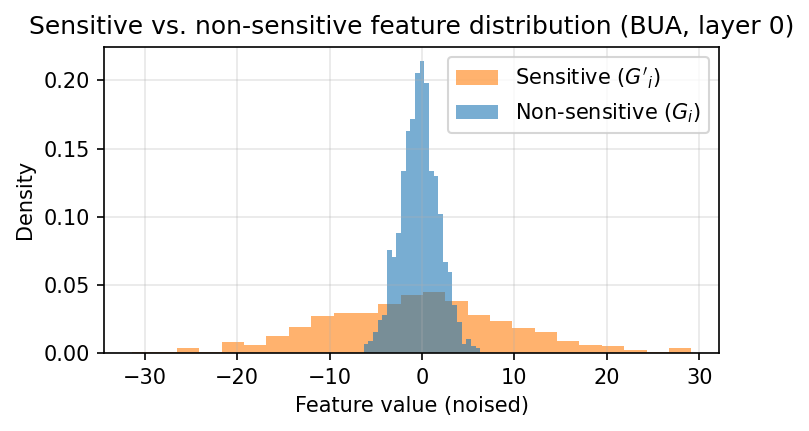
\includegraphics[width=0.95\columnwidth]{images/bodhi_vlm_sensitive_dist.png}
\caption{Sensitive vs.\ non-sensitive feature distribution (BUA, layer 0; noised features).}
\label{fig:sensitive_dist}
\end{figure}

\begin{figure}[t]
\centering
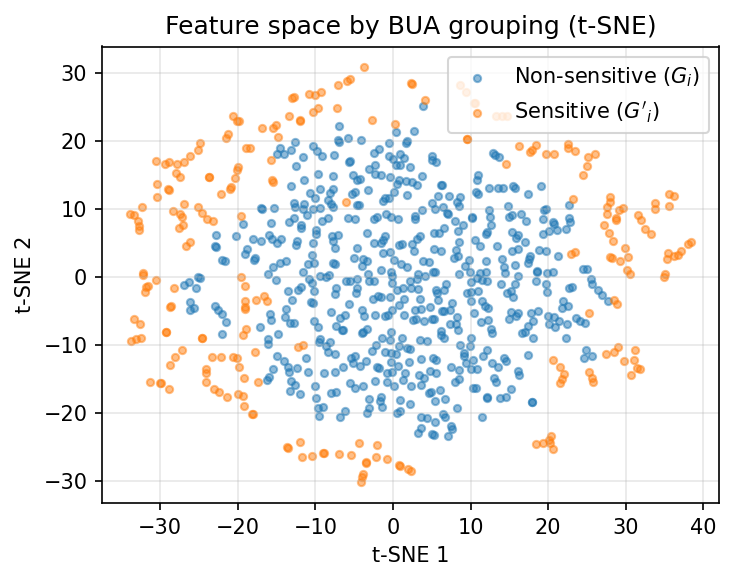
\includegraphics[width=0.95\columnwidth]{images/bodhi_vlm_tsne.png}
\caption{t-SNE (or PCA) of layer-wise features colored by BUA grouping: sensitive ($G'_i$) vs.\ non-sensitive ($G_i$).}
\label{fig:tsne}
\end{figure}

\section{Conclusion}
\label{sec:conclusion}

We presented Bodhi VLM, a privacy budget assessment framework that combines a bottom-up feature search (BUA), a top-down feature search (TDA), and an Expectation-Maximization Privacy Assessment (EMPA) module. The same pipeline applies to object detectors with feature pyramid backbones and to the vision towers of vision-language models such as CLIP, LLaVA, and BLIP. We contrasted Bodhi VLM with representative VLM privacy methods (ViP, DP-Cap, DP-MTV, VisShield) and showed that EMPA attains lower rMSE when assessing budget alignment on CLIP and LLaVA vision features. BUA and TDA produce layer-wise sensitive and non-sensitive feature groups; EMPA reconstructs the privacy-feature distribution and outputs a bias relative to the declared budget. On MOT20 and COCO, BUA and TDA exhibit similar deviation trends, with BUA slightly more sensitive to injected noise, and EMPA yields lower rMSE than Chi-square, K-L divergence, and MMD. We also provided an experimental protocol and accompanying code that enable reproducible evaluation. Future work includes integrating Bodhi VLM into full VLM training pipelines, developing one-shot auditing procedures, comparing against theoretical lower bounds on information leakage, and designing automated feedback mechanisms to adaptively tune $\epsilon$ at the preprocessing layer.

\bibliographystyle{IEEEtran}
\bibliography{ref}

\end{document}
